\documentclass[a4paper]{book}
\usepackage{makeidx}
\usepackage{graphicx}
\usepackage{multicol}
\usepackage{float}
\usepackage{listings}
\usepackage{color}
\usepackage{ifthen}
\usepackage[table]{xcolor}
\usepackage{textcomp}
\usepackage{alltt}
\usepackage{ifpdf}
\ifpdf
\usepackage[pdftex,
            pagebackref=true,
            colorlinks=true,
            linkcolor=blue,
            unicode
           ]{hyperref}
\else
\usepackage[ps2pdf,
            pagebackref=true,
            colorlinks=true,
            linkcolor=blue,
            unicode
           ]{hyperref}
\usepackage{pspicture}
\fi
\usepackage[utf8]{inputenc}
\usepackage{mathptmx}
\usepackage[scaled=.90]{helvet}
\usepackage{courier}
\usepackage{doxygen}
\lstset{language=C++,inputencoding=utf8,basicstyle=\footnotesize,breaklines=true,breakatwhitespace=true,tabsize=8,numbers=left }
\makeindex
\setcounter{tocdepth}{3}
\renewcommand{\footrulewidth}{0.4pt}
\begin{document}
\hypersetup{pageanchor=false}
\begin{titlepage}
\vspace*{7cm}
\begin{center}
{\Large RGine \\[1ex]\large 0.1 }\\
\vspace*{1cm}
{\large Generated by Doxygen 1.7.3}\\
\vspace*{0.5cm}
{\small Thu Aug 4 2011 09:11:27}\\
\end{center}
\end{titlepage}
\clearemptydoublepage
\pagenumbering{roman}
\tableofcontents
\clearemptydoublepage
\pagenumbering{arabic}
\hypersetup{pageanchor=true}
\chapter{Class Index}
\section{Class Hierarchy}
This inheritance list is sorted roughly, but not completely, alphabetically:\begin{DoxyCompactList}
\item \contentsline{section}{KeyStruct}{\pageref{structKeyStruct}}{}
\item \contentsline{section}{MouseStruct}{\pageref{structMouseStruct}}{}
\item \contentsline{section}{RColor}{\pageref{classRColor}}{}
\item \contentsline{section}{REntity}{\pageref{classREntity}}{}
\item \contentsline{section}{RFrame}{\pageref{classRFrame}}{}
\item \contentsline{section}{RGLText}{\pageref{classRGLText}}{}
\item \contentsline{section}{RList$<$ T $>$}{\pageref{classRList}}{}
\item \contentsline{section}{RMain}{\pageref{classRMain}}{}
\begin{DoxyCompactList}
\item \contentsline{section}{Game}{\pageref{classGame}}{}
\end{DoxyCompactList}
\item \contentsline{section}{RPhysicalObject}{\pageref{classRPhysicalObject}}{}
\item \contentsline{section}{RPoint2i}{\pageref{classRPoint2i}}{}
\item \contentsline{section}{RPoint3f}{\pageref{classRPoint3f}}{}
\item \contentsline{section}{RSDL}{\pageref{classRSDL}}{}
\item \contentsline{section}{RString}{\pageref{classRString}}{}
\item \contentsline{section}{RTriMesh}{\pageref{classRTriMesh}}{}
\item \contentsline{section}{RVector}{\pageref{classRVector}}{}
\end{DoxyCompactList}

\chapter{Class Index}
\section{Class List}
Here are the classes, structs, unions and interfaces with brief descriptions:\begin{DoxyCompactList}
\item\contentsline{section}{\hyperlink{classGame}{Game} }{\pageref{classGame}}{}
\item\contentsline{section}{\hyperlink{structKeyStruct}{KeyStruct} }{\pageref{structKeyStruct}}{}
\item\contentsline{section}{\hyperlink{structMouseStruct}{MouseStruct} }{\pageref{structMouseStruct}}{}
\item\contentsline{section}{\hyperlink{classRColor}{RColor} }{\pageref{classRColor}}{}
\item\contentsline{section}{\hyperlink{classREntity}{REntity} }{\pageref{classREntity}}{}
\item\contentsline{section}{\hyperlink{classRFrame}{RFrame} }{\pageref{classRFrame}}{}
\item\contentsline{section}{\hyperlink{classRGLText}{RGLText} }{\pageref{classRGLText}}{}
\item\contentsline{section}{\hyperlink{classRList}{RList$<$ T $>$} }{\pageref{classRList}}{}
\item\contentsline{section}{\hyperlink{classRMain}{RMain} }{\pageref{classRMain}}{}
\item\contentsline{section}{\hyperlink{classRPhysicalObject}{RPhysicalObject} }{\pageref{classRPhysicalObject}}{}
\item\contentsline{section}{\hyperlink{classRPoint2i}{RPoint2i} }{\pageref{classRPoint2i}}{}
\item\contentsline{section}{\hyperlink{classRPoint3f}{RPoint3f} }{\pageref{classRPoint3f}}{}
\item\contentsline{section}{\hyperlink{classRSDL}{RSDL} }{\pageref{classRSDL}}{}
\item\contentsline{section}{\hyperlink{classRString}{RString} }{\pageref{classRString}}{}
\item\contentsline{section}{\hyperlink{classRTriMesh}{RTriMesh} }{\pageref{classRTriMesh}}{}
\item\contentsline{section}{\hyperlink{classRVector}{RVector} }{\pageref{classRVector}}{}
\end{DoxyCompactList}

\chapter{Class Documentation}
\hypertarget{classGame}{
\section{Game Class Reference}
\label{classGame}\index{Game@{Game}}
}
Inheritance diagram for Game:\begin{figure}[H]
\begin{center}
\leavevmode
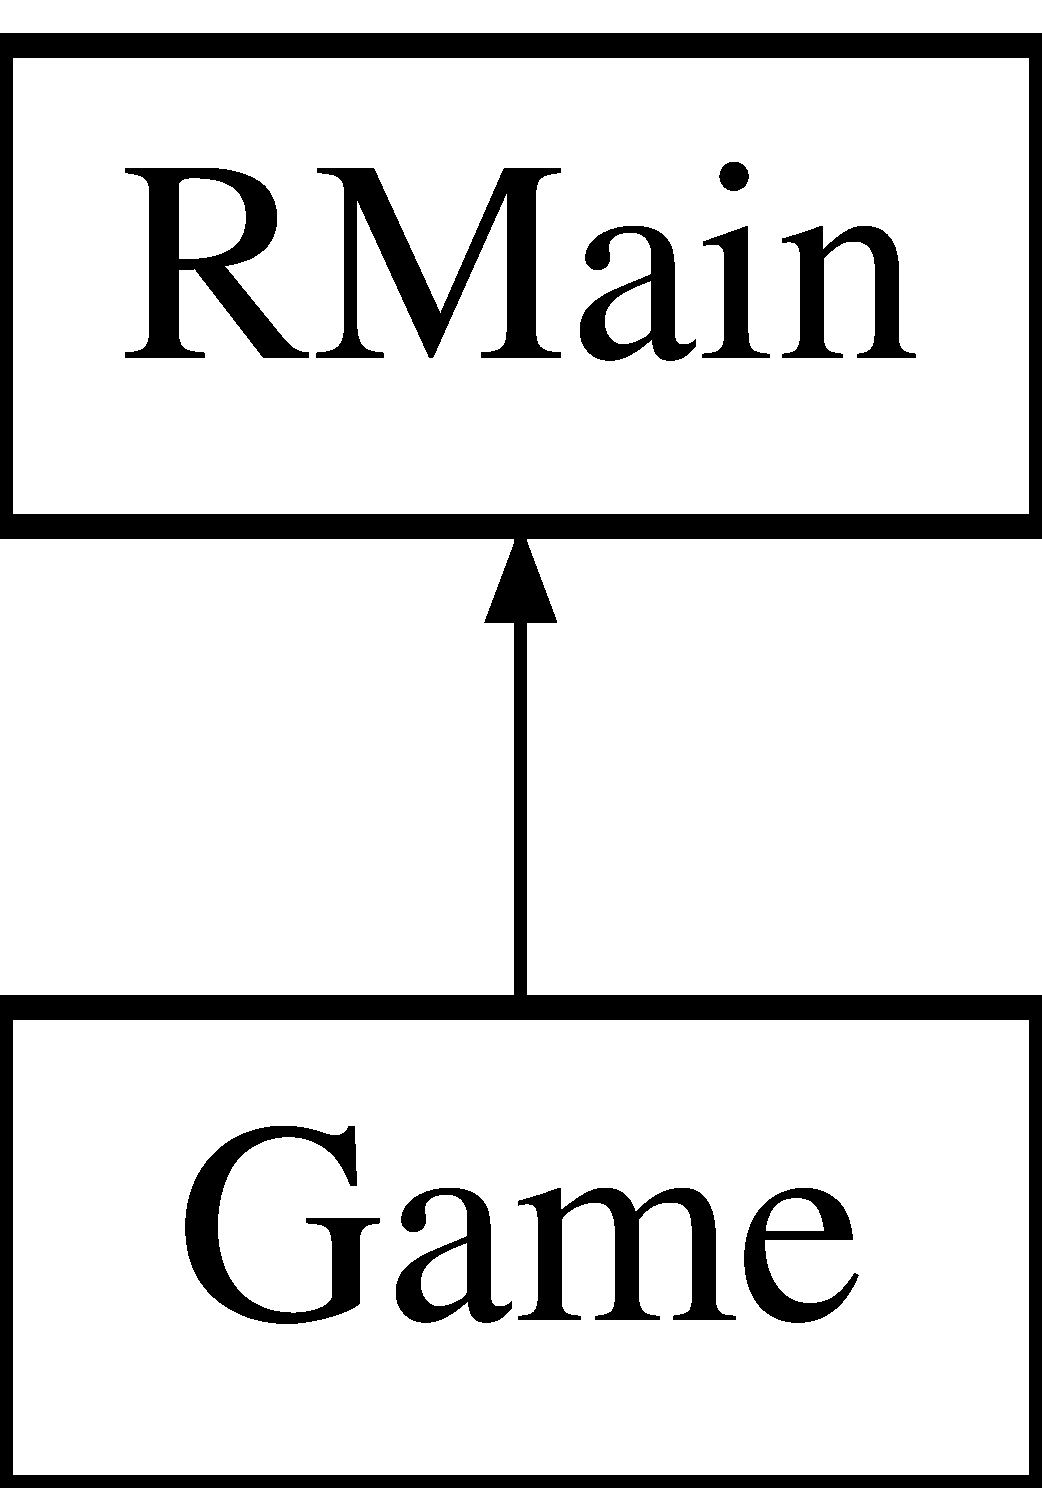
\includegraphics[height=2.000000cm]{classGame}
\end{center}
\end{figure}
\subsection*{Public Member Functions}
\begin{DoxyCompactItemize}
\item 
\hypertarget{classGame_a6f3a33940524b6ba9d83f627ccb14bbf}{
void {\bfseries init} ()}
\label{classGame_a6f3a33940524b6ba9d83f627ccb14bbf}

\item 
\hypertarget{classGame_ae93d6615d19503966f6e20235adc6daf}{
void {\bfseries logic} ()}
\label{classGame_ae93d6615d19503966f6e20235adc6daf}

\item 
\hypertarget{classGame_a15ddd769261d923827a3cdf41499c843}{
void {\bfseries render} ()}
\label{classGame_a15ddd769261d923827a3cdf41499c843}

\end{DoxyCompactItemize}


The documentation for this class was generated from the following files:\begin{DoxyCompactItemize}
\item 
Game.h\item 
Game.cpp\end{DoxyCompactItemize}

\hypertarget{structKeyStruct}{
\section{KeyStruct Struct Reference}
\label{structKeyStruct}\index{KeyStruct@{KeyStruct}}
}
\subsection*{Public Attributes}
\begin{DoxyCompactItemize}
\item 
\hypertarget{structKeyStruct_a91817c04bbf451a28fd5de1c9086d21e}{
bool {\bfseries up}}
\label{structKeyStruct_a91817c04bbf451a28fd5de1c9086d21e}

\item 
\hypertarget{structKeyStruct_a3dafff3adbc49fa64615328147c2a13c}{
bool {\bfseries down}}
\label{structKeyStruct_a3dafff3adbc49fa64615328147c2a13c}

\item 
\hypertarget{structKeyStruct_ae3308f8d6913936ba151ac9d57bb97bd}{
bool {\bfseries isDown}}
\label{structKeyStruct_ae3308f8d6913936ba151ac9d57bb97bd}

\end{DoxyCompactItemize}


The documentation for this struct was generated from the following file:\begin{DoxyCompactItemize}
\item 
engine/include/RSDL.h\end{DoxyCompactItemize}

\hypertarget{structMouseStruct}{
\section{MouseStruct Struct Reference}
\label{structMouseStruct}\index{MouseStruct@{MouseStruct}}
}
\subsection*{Public Attributes}
\begin{DoxyCompactItemize}
\item 
\hypertarget{structMouseStruct_a251ff02d33b9903cb5cd8f9e33590ec4}{
\hyperlink{structKeyStruct}{KeyStruct} {\bfseries left}}
\label{structMouseStruct_a251ff02d33b9903cb5cd8f9e33590ec4}

\item 
\hypertarget{structMouseStruct_a9648c56a8f1c04c3ca39b6dae930a26e}{
\hyperlink{structKeyStruct}{KeyStruct} {\bfseries right}}
\label{structMouseStruct_a9648c56a8f1c04c3ca39b6dae930a26e}

\item 
\hypertarget{structMouseStruct_a0533f4e13a240426a1deb0f92e7c3cc7}{
\hyperlink{structKeyStruct}{KeyStruct} {\bfseries middle}}
\label{structMouseStruct_a0533f4e13a240426a1deb0f92e7c3cc7}

\item 
\hypertarget{structMouseStruct_ad25364a6968748180cd20868c9765d68}{
\hyperlink{structKeyStruct}{KeyStruct} {\bfseries wheelup}}
\label{structMouseStruct_ad25364a6968748180cd20868c9765d68}

\item 
\hypertarget{structMouseStruct_ac642c0db4c6a27c49e2642a7182fb476}{
\hyperlink{structKeyStruct}{KeyStruct} {\bfseries wheeldown}}
\label{structMouseStruct_ac642c0db4c6a27c49e2642a7182fb476}

\item 
\hypertarget{structMouseStruct_a409dc6ce16cb1cc2615cfc0c8a715918}{
\hyperlink{classRPoint2i}{RPoint2i} {\bfseries position}}
\label{structMouseStruct_a409dc6ce16cb1cc2615cfc0c8a715918}

\item 
\hypertarget{structMouseStruct_af080e59430def924714674365454f8a3}{
\hyperlink{classRPoint2i}{RPoint2i} {\bfseries speed}}
\label{structMouseStruct_af080e59430def924714674365454f8a3}

\item 
\hypertarget{structMouseStruct_a7c167349789bcef4717211ad360a6d69}{
\hyperlink{classRPoint2i}{RPoint2i} {\bfseries wheelspeed}}
\label{structMouseStruct_a7c167349789bcef4717211ad360a6d69}

\end{DoxyCompactItemize}


The documentation for this struct was generated from the following file:\begin{DoxyCompactItemize}
\item 
engine/include/RSDL.h\end{DoxyCompactItemize}

\hypertarget{classRColor}{
\section{RColor Class Reference}
\label{classRColor}\index{RColor@{RColor}}
}
\subsection*{Public Member Functions}
\begin{DoxyCompactItemize}
\item 
\hypertarget{classRColor_a6d57b333fe49147d4b43c50bf1b293f8}{
{\bfseries RColor} (int r, int g, int b)}
\label{classRColor_a6d57b333fe49147d4b43c50bf1b293f8}

\item 
\hypertarget{classRColor_a408c595f2c0253bd9b1de992c5465c18}{
{\bfseries RColor} (float r, float g, float b)}
\label{classRColor_a408c595f2c0253bd9b1de992c5465c18}

\item 
\hypertarget{classRColor_a5d173c9122f07fd36228fee3604f46bf}{
int {\bfseries r} ()}
\label{classRColor_a5d173c9122f07fd36228fee3604f46bf}

\item 
\hypertarget{classRColor_aff6471bd0b53bc003059c72d15c5ea43}{
int {\bfseries g} ()}
\label{classRColor_aff6471bd0b53bc003059c72d15c5ea43}

\item 
\hypertarget{classRColor_a9dc9de4130f100ebdd49ebf0e7f89cb7}{
int {\bfseries b} ()}
\label{classRColor_a9dc9de4130f100ebdd49ebf0e7f89cb7}

\item 
\hypertarget{classRColor_a4d7b5a3e3f3fce0fd37d1157caeba77a}{
void {\bfseries setR} (int r)}
\label{classRColor_a4d7b5a3e3f3fce0fd37d1157caeba77a}

\item 
\hypertarget{classRColor_a9e099175f3a28b2fd7bba213eb9156bc}{
void {\bfseries setG} (int g)}
\label{classRColor_a9e099175f3a28b2fd7bba213eb9156bc}

\item 
\hypertarget{classRColor_a3bc3ded31002c363053788592270247e}{
void {\bfseries setB} (int b)}
\label{classRColor_a3bc3ded31002c363053788592270247e}

\item 
\hypertarget{classRColor_a6707fe3c885218ee8d4f1579df405181}{
float {\bfseries rF} ()}
\label{classRColor_a6707fe3c885218ee8d4f1579df405181}

\item 
\hypertarget{classRColor_af820dc92dbc8982dfba4419a5e5c6346}{
float {\bfseries gF} ()}
\label{classRColor_af820dc92dbc8982dfba4419a5e5c6346}

\item 
\hypertarget{classRColor_a31b431b26b651eaef114f31f29a87e79}{
float {\bfseries bF} ()}
\label{classRColor_a31b431b26b651eaef114f31f29a87e79}

\item 
\hypertarget{classRColor_a620c88b0ecfc6aeb6e3be308c53a223d}{
void {\bfseries setR} (float r)}
\label{classRColor_a620c88b0ecfc6aeb6e3be308c53a223d}

\item 
\hypertarget{classRColor_aaa40dfb82786e861b8695daf67426638}{
void {\bfseries setG} (float g)}
\label{classRColor_aaa40dfb82786e861b8695daf67426638}

\item 
\hypertarget{classRColor_aa1d520093061ef8780ca45ead346fb11}{
void {\bfseries setB} (float b)}
\label{classRColor_aa1d520093061ef8780ca45ead346fb11}

\end{DoxyCompactItemize}


The documentation for this class was generated from the following files:\begin{DoxyCompactItemize}
\item 
graphics/include/RColor.h\item 
graphics/src/RColor.cpp\end{DoxyCompactItemize}

\hypertarget{classREntity}{
\section{REntity Class Reference}
\label{classREntity}\index{REntity@{REntity}}
}
\subsection*{Public Member Functions}
\begin{DoxyCompactItemize}
\item 
\hypertarget{classREntity_a1a584b097fc46b6441f214cf99221b07}{
void {\bfseries handle} ()}
\label{classREntity_a1a584b097fc46b6441f214cf99221b07}

\end{DoxyCompactItemize}


The documentation for this class was generated from the following files:\begin{DoxyCompactItemize}
\item 
engine/include/REntity.h\item 
engine/src/REntity.cpp\end{DoxyCompactItemize}

\hypertarget{classRFrame}{
\section{RFrame Class Reference}
\label{classRFrame}\index{RFrame@{RFrame}}
}
\subsection*{Public Member Functions}
\begin{DoxyCompactItemize}
\item 
\hypertarget{classRFrame_aa925b91df1ddc68b1a6c1a5cc3bbad9a}{
void {\bfseries setIdentity} ()}
\label{classRFrame_aa925b91df1ddc68b1a6c1a5cc3bbad9a}

\item 
\hypertarget{classRFrame_a8a881dd99cdaed03a7c9df538a1a3d44}{
void {\bfseries setPosition} (float x, float y, float z)}
\label{classRFrame_a8a881dd99cdaed03a7c9df538a1a3d44}

\item 
\hypertarget{classRFrame_a9e5f303d1e292f7d2c4e4395ad40f846}{
void {\bfseries move} (float x, float y, float z)}
\label{classRFrame_a9e5f303d1e292f7d2c4e4395ad40f846}

\item 
\hypertarget{classRFrame_abdc72d6aa2057af096dcfb5fca98020c}{
void {\bfseries scale} (float x, float y, float z)}
\label{classRFrame_abdc72d6aa2057af096dcfb5fca98020c}

\item 
\hypertarget{classRFrame_a6d78d899004ce9cfdefdcae5bd5efc35}{
void {\bfseries rotate} (float angle, float x, float y, float z)}
\label{classRFrame_a6d78d899004ce9cfdefdcae5bd5efc35}

\item 
\hypertarget{classRFrame_a7a7b42fff68985d3059f9df0e2774e63}{
float $\ast$ {\bfseries getMatrix} ()}
\label{classRFrame_a7a7b42fff68985d3059f9df0e2774e63}

\end{DoxyCompactItemize}


The documentation for this class was generated from the following files:\begin{DoxyCompactItemize}
\item 
math/include/RFrame.h\item 
math/src/RFrame.cpp\end{DoxyCompactItemize}

\hypertarget{classRGLText}{
\section{RGLText Class Reference}
\label{classRGLText}\index{RGLText@{RGLText}}
}


The documentation for this class was generated from the following files:\begin{DoxyCompactItemize}
\item 
opengl/include/RGLText.h\item 
opengl/src/RGLText.cpp\end{DoxyCompactItemize}

\hypertarget{classRList}{
\section{RList$<$ T $>$ Class Template Reference}
\label{classRList}\index{RList@{RList}}
}
\subsection*{Public Member Functions}
\begin{DoxyCompactItemize}
\item 
\hypertarget{classRList_a5d999d1f42d4c5be12913570966ef21b}{
T {\bfseries operator\mbox{[}$\,$\mbox{]}} (const int index)}
\label{classRList_a5d999d1f42d4c5be12913570966ef21b}

\end{DoxyCompactItemize}
\subsubsection*{template$<$class T$>$ class RList$<$ T $>$}



The documentation for this class was generated from the following files:\begin{DoxyCompactItemize}
\item 
structures/include/RList.h\item 
structures/src/RList.cpp\end{DoxyCompactItemize}

\hypertarget{classRMain}{
\section{RMain Class Reference}
\label{classRMain}\index{RMain@{RMain}}
}
Inheritance diagram for RMain:\begin{figure}[H]
\begin{center}
\leavevmode
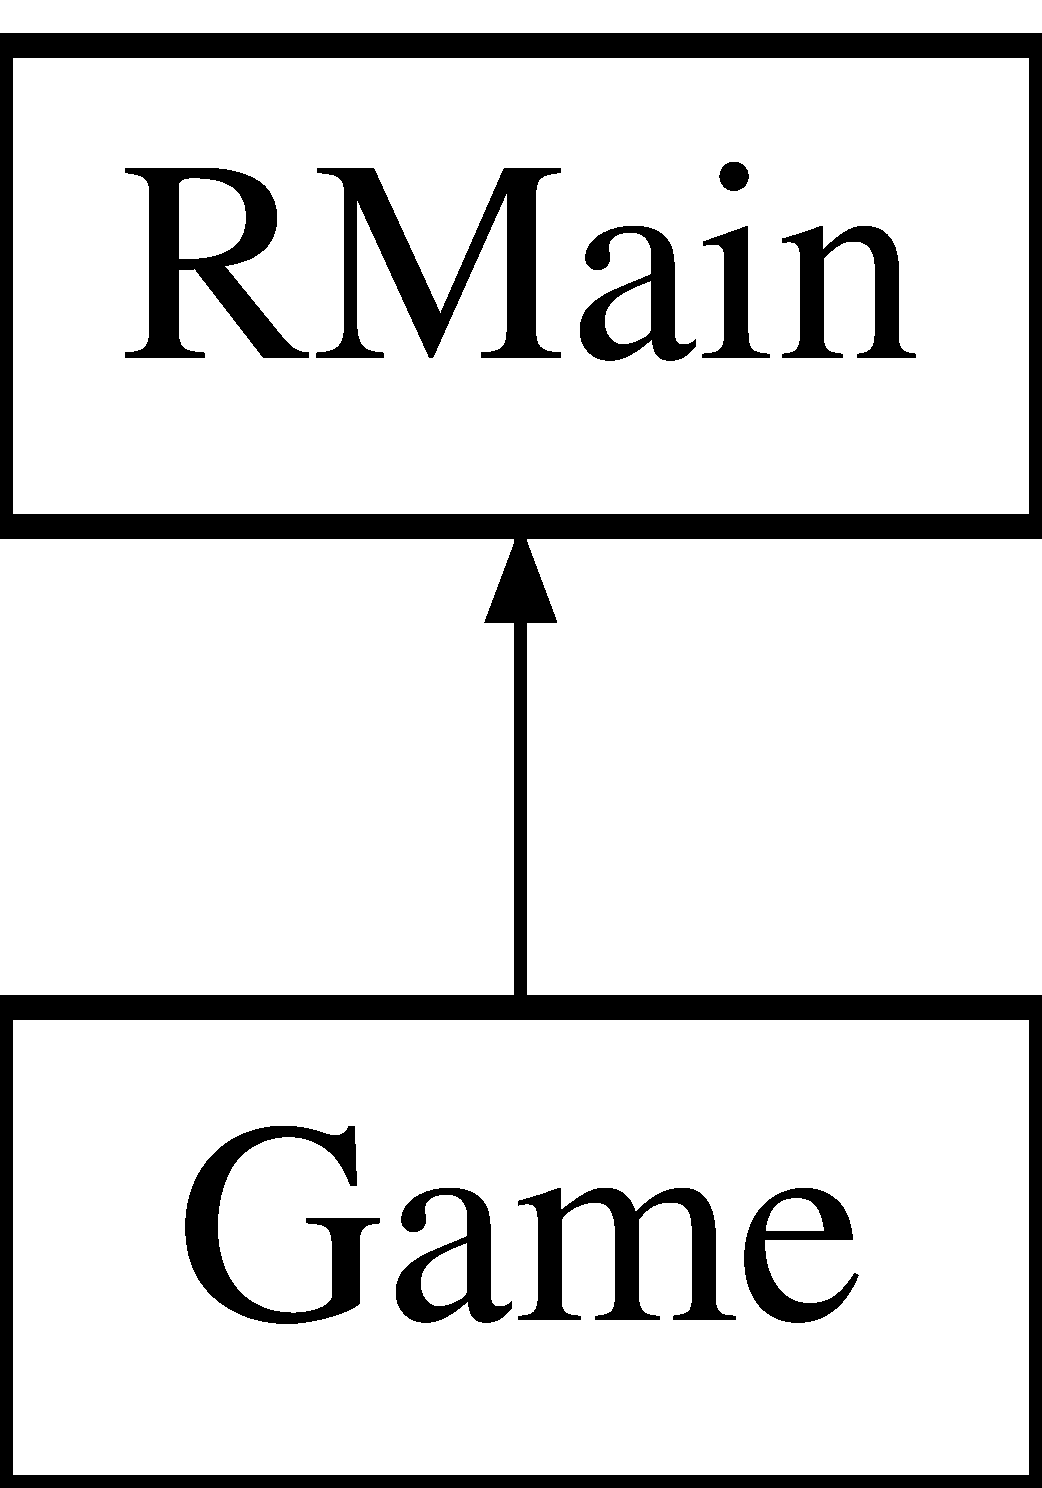
\includegraphics[height=2.000000cm]{classRMain}
\end{center}
\end{figure}
\subsection*{Public Member Functions}
\begin{DoxyCompactItemize}
\item 
\hypertarget{classRMain_a13a0972379c50832f3fde750043774c0}{
int {\bfseries run} ()}
\label{classRMain_a13a0972379c50832f3fde750043774c0}

\end{DoxyCompactItemize}
\subsection*{Protected Member Functions}
\begin{DoxyCompactItemize}
\item 
\hypertarget{classRMain_a3152809f7275f2f22901f0ce324ca8a8}{
\hyperlink{structMouseStruct}{MouseStruct} {\bfseries mouse} ()}
\label{classRMain_a3152809f7275f2f22901f0ce324ca8a8}

\item 
\hypertarget{classRMain_af59e77996c7aab57266de8caf93d2507}{
\hyperlink{structKeyStruct}{KeyStruct} {\bfseries key} (int id)}
\label{classRMain_af59e77996c7aab57266de8caf93d2507}

\end{DoxyCompactItemize}
\subsection*{Protected Attributes}
\begin{DoxyCompactItemize}
\item 
\hypertarget{classRMain_a029221b02c334c092cf86983e44b8231}{
\hyperlink{classRSDL}{RSDL} {\bfseries sdl}}
\label{classRMain_a029221b02c334c092cf86983e44b8231}

\end{DoxyCompactItemize}


The documentation for this class was generated from the following files:\begin{DoxyCompactItemize}
\item 
engine/include/RMain.h\item 
engine/src/RMain.cpp\end{DoxyCompactItemize}

\hypertarget{classRPhysicalObject}{
\section{RPhysicalObject Class Reference}
\label{classRPhysicalObject}\index{RPhysicalObject@{RPhysicalObject}}
}


The documentation for this class was generated from the following files:\begin{DoxyCompactItemize}
\item 
physics/include/RPhysicalObject.h\item 
physics/src/RPhysicalObject.cpp\end{DoxyCompactItemize}

\hypertarget{classRPoint2i}{
\section{RPoint2i Class Reference}
\label{classRPoint2i}\index{RPoint2i@{RPoint2i}}
}
\subsection*{Public Member Functions}
\begin{DoxyCompactItemize}
\item 
\hypertarget{classRPoint2i_aa4feadb6fd1a325999992eb3a848833f}{
{\bfseries RPoint2i} (int x, int y)}
\label{classRPoint2i_aa4feadb6fd1a325999992eb3a848833f}

\item 
\hypertarget{classRPoint2i_aa4eb37808d3385eabd7b7afcea2e51a0}{
int {\bfseries x} ()}
\label{classRPoint2i_aa4eb37808d3385eabd7b7afcea2e51a0}

\item 
\hypertarget{classRPoint2i_a8bd8470c25a32cd8294d8c48d61caddd}{
int {\bfseries y} ()}
\label{classRPoint2i_a8bd8470c25a32cd8294d8c48d61caddd}

\item 
\hypertarget{classRPoint2i_a632d2f16ae8af7b8f005788cda24300f}{
void {\bfseries setX} (int)}
\label{classRPoint2i_a632d2f16ae8af7b8f005788cda24300f}

\item 
\hypertarget{classRPoint2i_abe152656ead3df5f1d66e0bfa029ecdc}{
void {\bfseries setY} (int)}
\label{classRPoint2i_abe152656ead3df5f1d66e0bfa029ecdc}

\item 
\hypertarget{classRPoint2i_adc82f0451699260019d1e1acd296803a}{
void {\bfseries set} (int x, int y)}
\label{classRPoint2i_adc82f0451699260019d1e1acd296803a}

\item 
\hypertarget{classRPoint2i_aec6c8fd14340ded637491d808df04546}{
bool {\bfseries operator==} (\hyperlink{classRPoint2i}{RPoint2i})}
\label{classRPoint2i_aec6c8fd14340ded637491d808df04546}

\item 
\hypertarget{classRPoint2i_a610eabfd188b74ffb61cd446bcf79e3f}{
\hyperlink{classRPoint2i}{RPoint2i} {\bfseries operator=} (\hyperlink{classRPoint2i}{RPoint2i})}
\label{classRPoint2i_a610eabfd188b74ffb61cd446bcf79e3f}

\item 
\hypertarget{classRPoint2i_a71d9ed3107344a67cd5a4517252f47f0}{
\hyperlink{classRPoint2i}{RPoint2i} {\bfseries operator+} (\hyperlink{classRPoint2i}{RPoint2i})}
\label{classRPoint2i_a71d9ed3107344a67cd5a4517252f47f0}

\item 
\hypertarget{classRPoint2i_ad5b55b678d2a186b6a796493cadef4f2}{
\hyperlink{classRPoint2i}{RPoint2i} {\bfseries operator-\/} (\hyperlink{classRPoint2i}{RPoint2i})}
\label{classRPoint2i_ad5b55b678d2a186b6a796493cadef4f2}

\item 
\hypertarget{classRPoint2i_ad91208629c87ccab23588c055472c869}{
\hyperlink{classRPoint2i}{RPoint2i} {\bfseries operator$\ast$} (\hyperlink{classRPoint2i}{RPoint2i})}
\label{classRPoint2i_ad91208629c87ccab23588c055472c869}

\item 
\hypertarget{classRPoint2i_ae5c04de1a59c76da04245330e8729c6a}{
\hyperlink{classRPoint2i}{RPoint2i} {\bfseries operator$^\wedge$} (\hyperlink{classRPoint2i}{RPoint2i})}
\label{classRPoint2i_ae5c04de1a59c76da04245330e8729c6a}

\item 
\hypertarget{classRPoint2i_a8195aab0a1b1d0faf82a80f5feceefad}{
\hyperlink{classRPoint2i}{RPoint2i} {\bfseries operator$\ast$} (int)}
\label{classRPoint2i_a8195aab0a1b1d0faf82a80f5feceefad}

\item 
\hypertarget{classRPoint2i_ab9d18c17616afe42cb28e53ebc1bf334}{
\hyperlink{classRPoint2i}{RPoint2i} {\bfseries operator/} (int)}
\label{classRPoint2i_ab9d18c17616afe42cb28e53ebc1bf334}

\end{DoxyCompactItemize}


The documentation for this class was generated from the following files:\begin{DoxyCompactItemize}
\item 
math/include/RPoint2i.h\item 
math/src/RPoint2i.cpp\end{DoxyCompactItemize}

\hypertarget{classRPoint3f}{
\section{RPoint3f Class Reference}
\label{classRPoint3f}\index{RPoint3f@{RPoint3f}}
}
\subsection*{Public Member Functions}
\begin{DoxyCompactItemize}
\item 
\hypertarget{classRPoint3f_a31a47d79675ee201428f46e5c2ee1dc2}{
{\bfseries RPoint3f} (float x, float y, float z)}
\label{classRPoint3f_a31a47d79675ee201428f46e5c2ee1dc2}

\item 
\hypertarget{classRPoint3f_adbf9bc217d5d17197082cde3e5a8515a}{
float {\bfseries x} ()}
\label{classRPoint3f_adbf9bc217d5d17197082cde3e5a8515a}

\item 
\hypertarget{classRPoint3f_a4c5630e38f3313b8065375a0760be67b}{
float {\bfseries y} ()}
\label{classRPoint3f_a4c5630e38f3313b8065375a0760be67b}

\item 
\hypertarget{classRPoint3f_a89a8e4994236fd856bed8155ff694b89}{
float {\bfseries z} ()}
\label{classRPoint3f_a89a8e4994236fd856bed8155ff694b89}

\item 
\hypertarget{classRPoint3f_a87d08a6b3fb874eedb2a98782196bce9}{
void {\bfseries setX} (float x)}
\label{classRPoint3f_a87d08a6b3fb874eedb2a98782196bce9}

\item 
\hypertarget{classRPoint3f_a6fc795464d934d0a05b51c803893bb17}{
void {\bfseries setY} (float y)}
\label{classRPoint3f_a6fc795464d934d0a05b51c803893bb17}

\item 
\hypertarget{classRPoint3f_a8c09b32691638dd2b0fb80c4439f2fbb}{
void {\bfseries setZ} (float z)}
\label{classRPoint3f_a8c09b32691638dd2b0fb80c4439f2fbb}

\item 
\hypertarget{classRPoint3f_a539e6a17e802c3223034619cf2a7a366}{
void {\bfseries set} (float x, float y, float z)}
\label{classRPoint3f_a539e6a17e802c3223034619cf2a7a366}

\item 
\hypertarget{classRPoint3f_a1d650d3290d84cc525c2727f84a41df4}{
vector$<$ float $>$ {\bfseries getVector} ()}
\label{classRPoint3f_a1d650d3290d84cc525c2727f84a41df4}

\item 
\hypertarget{classRPoint3f_a7d3dc33322ba79659daa4d02bd638231}{
bool {\bfseries operator==} (\hyperlink{classRPoint3f}{RPoint3f})}
\label{classRPoint3f_a7d3dc33322ba79659daa4d02bd638231}

\item 
\hypertarget{classRPoint3f_a91a5fcb19d59ef764c8ef880d44f07a2}{
\hyperlink{classRPoint3f}{RPoint3f} {\bfseries operator=} (\hyperlink{classRPoint3f}{RPoint3f})}
\label{classRPoint3f_a91a5fcb19d59ef764c8ef880d44f07a2}

\item 
\hypertarget{classRPoint3f_a0a5cb6413150dca3617c3a60acc6a804}{
\hyperlink{classRPoint3f}{RPoint3f} {\bfseries operator+} (\hyperlink{classRPoint3f}{RPoint3f})}
\label{classRPoint3f_a0a5cb6413150dca3617c3a60acc6a804}

\item 
\hypertarget{classRPoint3f_ad8b3f62c25d59f8a57918e972023ecca}{
\hyperlink{classRPoint3f}{RPoint3f} {\bfseries operator-\/} (\hyperlink{classRPoint3f}{RPoint3f})}
\label{classRPoint3f_ad8b3f62c25d59f8a57918e972023ecca}

\item 
\hypertarget{classRPoint3f_ab1c9a33814f4592994f993bac8234056}{
\hyperlink{classRPoint3f}{RPoint3f} {\bfseries operator$\ast$} (\hyperlink{classRPoint3f}{RPoint3f})}
\label{classRPoint3f_ab1c9a33814f4592994f993bac8234056}

\item 
\hypertarget{classRPoint3f_ad0cf27c5b272bfd133f4eeac64cade75}{
\hyperlink{classRPoint3f}{RPoint3f} {\bfseries operator$^\wedge$} (\hyperlink{classRPoint3f}{RPoint3f})}
\label{classRPoint3f_ad0cf27c5b272bfd133f4eeac64cade75}

\item 
\hypertarget{classRPoint3f_aec443dc890e23a6440eaa21bfa5bada2}{
\hyperlink{classRPoint3f}{RPoint3f} {\bfseries operator$\ast$} (float)}
\label{classRPoint3f_aec443dc890e23a6440eaa21bfa5bada2}

\item 
\hypertarget{classRPoint3f_a8fe175bfa0da1cb9369933efc4d900bc}{
\hyperlink{classRPoint3f}{RPoint3f} {\bfseries operator/} (float)}
\label{classRPoint3f_a8fe175bfa0da1cb9369933efc4d900bc}

\item 
\hypertarget{classRPoint3f_aed67203068767ec502cd3844f79f8e04}{
bool {\bfseries compare} (\hyperlink{classRPoint3f}{RPoint3f})}
\label{classRPoint3f_aed67203068767ec502cd3844f79f8e04}

\item 
\hypertarget{classRPoint3f_a6490c717e4514d4f7c7d6f1f2b141901}{
\hyperlink{classRPoint3f}{RPoint3f} {\bfseries set} (\hyperlink{classRPoint3f}{RPoint3f})}
\label{classRPoint3f_a6490c717e4514d4f7c7d6f1f2b141901}

\item 
\hypertarget{classRPoint3f_a7339009c46035a33fe9d1c8a18229593}{
\hyperlink{classRPoint3f}{RPoint3f} {\bfseries add} (\hyperlink{classRPoint3f}{RPoint3f})}
\label{classRPoint3f_a7339009c46035a33fe9d1c8a18229593}

\item 
\hypertarget{classRPoint3f_a6d93150dd498def35debe62ee73d19c7}{
\hyperlink{classRPoint3f}{RPoint3f} {\bfseries subtract} (\hyperlink{classRPoint3f}{RPoint3f})}
\label{classRPoint3f_a6d93150dd498def35debe62ee73d19c7}

\item 
\hypertarget{classRPoint3f_a67434ef289db90de0b9c262863ccb047}{
\hyperlink{classRPoint3f}{RPoint3f} {\bfseries dotProduct} (\hyperlink{classRPoint3f}{RPoint3f})}
\label{classRPoint3f_a67434ef289db90de0b9c262863ccb047}

\item 
\hypertarget{classRPoint3f_a02e9e481d1845a008eb85fefe943d8f3}{
\hyperlink{classRPoint3f}{RPoint3f} {\bfseries crossProduct} (\hyperlink{classRPoint3f}{RPoint3f})}
\label{classRPoint3f_a02e9e481d1845a008eb85fefe943d8f3}

\item 
\hypertarget{classRPoint3f_a4be010ccc48b57c6c2c390ff6bc5ff8b}{
\hyperlink{classRPoint3f}{RPoint3f} {\bfseries multiply} (float)}
\label{classRPoint3f_a4be010ccc48b57c6c2c390ff6bc5ff8b}

\item 
\hypertarget{classRPoint3f_a98bedc2e2bd8c60809dcbb62e9040657}{
\hyperlink{classRPoint3f}{RPoint3f} {\bfseries divide} (float)}
\label{classRPoint3f_a98bedc2e2bd8c60809dcbb62e9040657}

\end{DoxyCompactItemize}


The documentation for this class was generated from the following files:\begin{DoxyCompactItemize}
\item 
math/include/RPoint3f.h\item 
math/src/RPoint3f.cpp\end{DoxyCompactItemize}

\hypertarget{classRSDL}{
\section{RSDL Class Reference}
\label{classRSDL}\index{RSDL@{RSDL}}
}
\subsection*{Public Member Functions}
\begin{DoxyCompactItemize}
\item 
\hypertarget{classRSDL_a1bf9913888b5c8a5cf3408d622fbc4c2}{
bool {\bfseries init} ()}
\label{classRSDL_a1bf9913888b5c8a5cf3408d622fbc4c2}

\item 
\hypertarget{classRSDL_af162a71862213d98bcf7c2c045b162f8}{
bool {\bfseries end} ()}
\label{classRSDL_af162a71862213d98bcf7c2c045b162f8}

\item 
\hypertarget{classRSDL_a42d46d15990b40c9f284c020c4b4a570}{
void {\bfseries timer\_\-init} ()}
\label{classRSDL_a42d46d15990b40c9f284c020c4b4a570}

\item 
\hypertarget{classRSDL_a5fe4f0e3ad791b582fed8036da944bb7}{
void {\bfseries timer\_\-start} ()}
\label{classRSDL_a5fe4f0e3ad791b582fed8036da944bb7}

\item 
\hypertarget{classRSDL_a019f225f982105d3baa7f3d531515bfa}{
void {\bfseries timer\_\-stop} ()}
\label{classRSDL_a019f225f982105d3baa7f3d531515bfa}

\item 
\hypertarget{classRSDL_a0d22c943a2153c17ea610ec2effe3a61}{
void {\bfseries timer\_\-pause} ()}
\label{classRSDL_a0d22c943a2153c17ea610ec2effe3a61}

\item 
\hypertarget{classRSDL_a9751e0e2414c8743539b0376215a047f}{
void {\bfseries timer\_\-unpause} ()}
\label{classRSDL_a9751e0e2414c8743539b0376215a047f}

\item 
\hypertarget{classRSDL_a7db68f9d5ed9f15976e7ba4829273927}{
void {\bfseries timer\_\-delay} ()}
\label{classRSDL_a7db68f9d5ed9f15976e7ba4829273927}

\item 
\hypertarget{classRSDL_a68f700744989ba43ff3885ce8a87cb7c}{
int {\bfseries timer\_\-getTicks} ()}
\label{classRSDL_a68f700744989ba43ff3885ce8a87cb7c}

\item 
\hypertarget{classRSDL_a4de7a39e0f460f4cd4906069cc0ada6a}{
bool {\bfseries finished} ()}
\label{classRSDL_a4de7a39e0f460f4cd4906069cc0ada6a}

\item 
\hypertarget{classRSDL_aeb7a11c46d1895d201770fa2b9625412}{
void {\bfseries input} ()}
\label{classRSDL_aeb7a11c46d1895d201770fa2b9625412}

\item 
\hypertarget{classRSDL_a0c253f055c7bd372df0ea6654cc0cb48}{
void {\bfseries render\_\-begin} ()}
\label{classRSDL_a0c253f055c7bd372df0ea6654cc0cb48}

\item 
\hypertarget{classRSDL_acda1a87cb1f0735565a38c1037d0eb90}{
void {\bfseries render\_\-end} ()}
\label{classRSDL_acda1a87cb1f0735565a38c1037d0eb90}

\item 
\hypertarget{classRSDL_a33ebb844ae21af49b4e704bb4f6e2602}{
\hyperlink{structMouseStruct}{MouseStruct} {\bfseries mouse} ()}
\label{classRSDL_a33ebb844ae21af49b4e704bb4f6e2602}

\item 
\hypertarget{classRSDL_a4c8d44cd6e6bf7c6a36d963f6a0c8ccf}{
\hyperlink{structKeyStruct}{KeyStruct} {\bfseries key} (int)}
\label{classRSDL_a4c8d44cd6e6bf7c6a36d963f6a0c8ccf}

\item 
\hypertarget{classRSDL_abd0fc4cb4d19b97b3fbc8b1fa104c3d5}{
int {\bfseries getWidth} ()}
\label{classRSDL_abd0fc4cb4d19b97b3fbc8b1fa104c3d5}

\item 
\hypertarget{classRSDL_ae961056a7ce7b421441f2c950df0e99e}{
int {\bfseries getHeight} ()}
\label{classRSDL_ae961056a7ce7b421441f2c950df0e99e}

\end{DoxyCompactItemize}


The documentation for this class was generated from the following files:\begin{DoxyCompactItemize}
\item 
engine/include/RSDL.h\item 
engine/src/RSDL.cpp\end{DoxyCompactItemize}

\hypertarget{classRString}{
\section{RString Class Reference}
\label{classRString}\index{RString@{RString}}
}


The documentation for this class was generated from the following files:\begin{DoxyCompactItemize}
\item 
structures/include/RString.h\item 
structures/src/RString.cpp\end{DoxyCompactItemize}

\hypertarget{classRTriMesh}{
\section{RTriMesh Class Reference}
\label{classRTriMesh}\index{RTriMesh@{RTriMesh}}
}
\subsection*{Public Member Functions}
\begin{DoxyCompactItemize}
\item 
\hypertarget{classRTriMesh_aa6fc41bb284fcf611407ba8a8eed6d2d}{
void {\bfseries addPoint} (\hyperlink{classRPoint3f}{RPoint3f} point, \hyperlink{classRPoint3f}{RPoint3f} normal, \hyperlink{classRColor}{RColor} color)}
\label{classRTriMesh_aa6fc41bb284fcf611407ba8a8eed6d2d}

\item 
\hypertarget{classRTriMesh_a4950038ac0141f177284a2defb22ae04}{
\hyperlink{classRPoint3f}{RPoint3f} {\bfseries getPoint} (int at)}
\label{classRTriMesh_a4950038ac0141f177284a2defb22ae04}

\item 
\hypertarget{classRTriMesh_a3e20aff5157c9b99d7ab6fa67dd83e33}{
void {\bfseries removePoint} (int at)}
\label{classRTriMesh_a3e20aff5157c9b99d7ab6fa67dd83e33}

\end{DoxyCompactItemize}


The documentation for this class was generated from the following files:\begin{DoxyCompactItemize}
\item 
structures/include/RTriMesh.h\item 
structures/src/RTriMesh.cpp\end{DoxyCompactItemize}

\hypertarget{classRVector}{
\section{RVector Class Reference}
\label{classRVector}\index{RVector@{RVector}}
}


The documentation for this class was generated from the following files:\begin{DoxyCompactItemize}
\item 
structures/include/RVector.h\item 
structures/src/RVector.cpp\end{DoxyCompactItemize}

\printindex
\end{document}
